\section{Installation and Start}
\label{installation}

Start off by downloading \bms~for your operating system. 
You can find the latest version of the tool at \url{http://www.stups.hhu.de/ProB/index.php5/BMotion_Studio}.
Decompress the archive and expand the directory if necessary. 

%\warning{Do not change the location and structure of the files and directories within the folder!}

Navigate to the \texttt{server/bin} folder and start the server by entering the bash command:

\begin{lstlisting}[language=bash]
.\standalone
\end{lstlisting}

\info{Windows users should execute the \texttt{standalone.bat} file.}

Now, navigate to the \texttt{client} folder and start the client by executing the \texttt{bmotion-prob} program.
The window shown in Figure~\ref{fig_bms_client} should popup.

\begin{figure}[!ht]
\begin{center}
	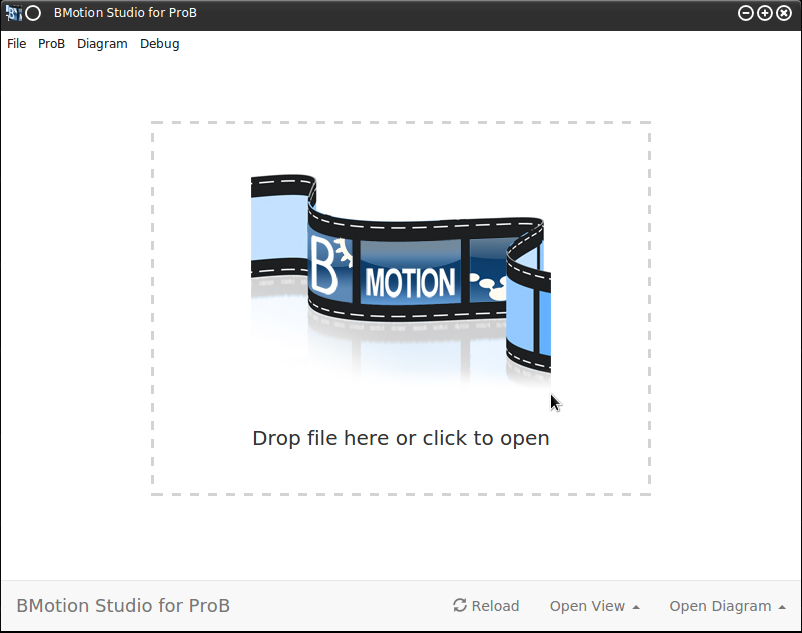
\includegraphics[width=\textwidth]{img/tutorial/clientstartscreen.png}
	\caption{\bms\ Client}
	\label{fig_bms_client}
\end{center}
\end{figure} 

%Your default browser should open and show the default workspace.
%The workspace contains the following predefined folders:
%\begin{itemize}
%\item \texttt{libs}: This folder contains JavaScript libraries that are needed for BMotion Studio.
%\item \texttt{b\_template}: A visualization template for creating visualizations for Classical-B and Event-B models.
%\item \texttt{csp\_template}: A visualization template for creating visualizations for CSP models.
%\end{itemize}

\section{Create a new Visualization Template}
\label{vis_template}

Let's start by creating a new visualization template.
The easiest way to create a new visualization template is to download the \file{bms-b-template.zip}{predefined template}.
Decompress the archive, expand the directory if necessary and navigate to the decompressed folder.
The folder contains some files:

%	duplicate one of the default templates  \texttt{b\_template} (for Event-B or Classical-B visualizations) or \texttt{csp\_template} (for CSP-M visualizations) that are included in the \texttt{workspace} folder of your \bms~installation.
%Just duplicate the folder.
%After refreshing your browser, the newly created folder should appear in your workspace.
%Navigate to the folder. 
%The folder contains three files.

%\paragraph{\texttt{template.groovy:}}
%The Groovy script file is the place where the user can communicate with the formal model by means of the ProB Java API\footnote{\url{http://www.stups.hhu.de/ProB/index.php5/ProB_Java_API}}.
%For instance, the user may register methods that can be called in the JavaScript w.
%The Groovy script file is the place where you can setup the communication between your visualization and the ProB animator.
%In particular, the Groovy script file is the link between the formal model and the visualization.
%It allows you to programmatically control the ProB animator and to access the actual formal model being visualised.

\paragraph{\texttt{bmotion.json:}}
The \texttt{bmotion.json} file is the root file of every \bms\ visualization.
It contains the configuration formatted using JSON (JavaScript Object Notation)\footnote{\url{http://www.json.org}.}.
The following options are available:

\begin{tabular}{ l l l p{7cm} }
  \textbf{Name} & \textbf{Type} & \textbf{Default} & \textbf{Description} \\
  \hline\noalign{\medskip}
  name & string & & The name of the visualization.\\
  \hline\noalign{\medskip}
  template* & string & & The relative path to the HTML visualization file. \\
  \hline\noalign{\medskip}
  model* & string & & The relative path to the model. \\
  \hline\noalign{\medskip}
  tool & string & BAnimation & The formalism / tool to be used. Currently two values are allowed: \textit{BAnimation} for creating visualizations of Event-B or Classical-B models and \textit{CSPAnimation} for creating visualizations of CSP-M models.\\
\end{tabular}

*These options are required.

\vspace*{0.5cm}

A minimal configuration of the \texttt{bmotion.json} file should contain the path to the template and the path to the model to be visualized.
Here is an example \texttt{bmotion.json} file with a minimal configuration:

\begin{lstlisting}[language=JavaScript]
{
  "template": "index.html",
  "model": "model/model.mch"
}
\end{lstlisting}


\paragraph{\texttt{script.js:}}
In the JavaScript file you can setup observers and actions (see Section~\ref{reference_b}).
Moreover, the user can take advantage of the entire JavaScript language.
There exist are a lot of libraries for JavaScript that you can apply to create custom visualizations.
For instance, it exists libraries for generating chart and plot diagrams.
%In addition, you can call functions that are registered in the Groovy script file.
%This enables you to add some interactivity to your visualization.
%For instance, pressing a button in your visualization could cause the execution of an Event-B event.
Here is an example \texttt{script.js} file with a minimal configuration:

\begin{lstlisting}[language=JavaScript]
requirejs(['bmotion.vis'], function () {
  // Put your code here
});
\end{lstlisting}

%The \textit{prob} parameter is the access point to the BMotion Studio for ProB API.

\paragraph{\texttt{index.html:}}
%The HTML file is the root file of your visualization. It contains the actual visualization.
The HTML file contains the actual visualization.
Here is an example \texttt{index.html} file with a minimal configuration:

\begin{lstlisting}[language=html]
<html data-bms-visualisation>
  <head>
    <title>BMotion Studio Visualization</title>
  </head>
  <body>
    <script data-main="script" src="require.js"></script>
  </body>
</html>
\end{lstlisting}

Please note the attribute \textit{data-bms-visualisation} in line 1.
Every \bms\ visualization template file should contain the empty attribute \textit{data-bms-visualisation}.
In addition, every \bms\ visualizations template file should contain a reference to your \texttt{scripts.js} file as demonstarted in line 7.

%The meta tag \textit{bms.tool} (line 4) defines the formalism or the simulator respectively that should be used. 
%Two values are allowed: ``BAnimation'' for creating visualizations of Event-B or Classical-B models and ``CSPAnimation'' for creating visualizations of CSP-M models.
%The meta tag \textit{bms.script} (line 5) contains the link to the Groovy script file.
%Finally, in line 9 we define the path to the JavaScript file.

The user is not restricted to an editor in order to create a visualization.
The user can make use of any tool that supports the creation of SVG graphics or HTML documents.
For the tutorials (Section~\ref{tutorial_b} and~\ref{tutorial_csp}) we are going to use the Inkspace\footnote{\url{https://inkscape.org}} editor. Inkscape is an editor for creating vector graphics that is available for Windows, Mac OS X and Linux.
It's free and open source.
With Inkscape the user can export the vector graphic into the SVG format.
The SVG code can then be included in the \texttt{index.html} file.

\begin{figure}[!ht]
\begin{center}
	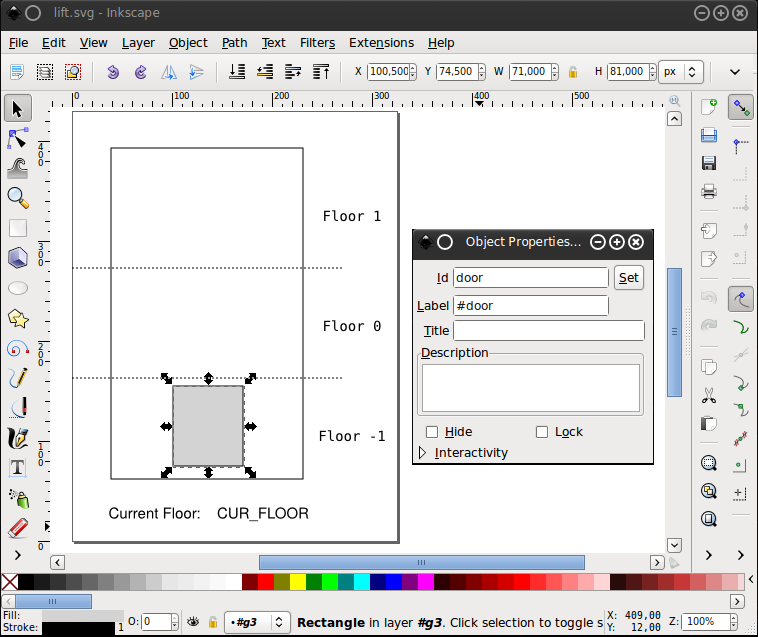
\includegraphics[width=12cm]{img/tutorial/tut_02.png}
	\caption{Creating an SVG graphic with Inkscape}
	\label{fig_tut_02_inkscape}
\end{center}
\end{figure} 

\paragraph{\texttt{bmotion.vis.js and require.js:}}
JavaScript libraries that are needed for running the visualization.
Please do not edit them!

%\section{Link a Model with a Visualization}
%
%In order to link a model with the visualization, open the \texttt{bmotion.json} file with an editor of your choice and adapt the \textit{model} property.
%The model \textit{model} property should contain the path to your model file (e.g. \texttt{mymodel/model.mch}).
%The model should be places relative to your bmotion.json file.
%Linking a model within the \texttt{bmotion.json} file will automatically load the model, when starting the visualization.

%To create a link between graphical elements and the model, please checkout the Section \ref{tutorial_b} for Event-B and Classical-B or \ref{tutorial_csp} for CSP.
